% Overleaf compiler: pdfLaTeX
\documentclass{article}
\usepackage{tikz}
\usetikzlibrary{arrows.meta,positioning}

\begin{document}
\section*{A small state machine}

Figure~\ref{fig:states} shows three states and the moves between them.

\begin{figure}[h]
  \centering
  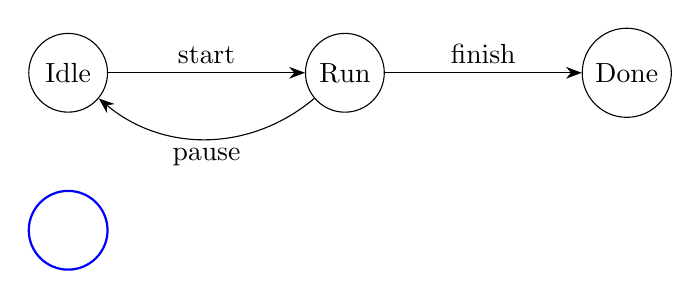
\begin{tikzpicture}[
      node distance=2.5cm,
      state/.style={circle, draw, minimum size=1cm},
      >={Stealth[length=2mm]}
    ]
    \node[state] (idle) {Idle};
    \node[state, right=of idle] (run) {Run};
    \node[state, right=of run] (done) {Done};
    \draw[->] (idle) -- node[above] {start} (run);
    \draw[->] (run) -- node[above] {finish} (done);
    \draw[->] (run) to[bend left=40] node[below] {pause} (idle);
    \draw[thick, blue] (0,-2) circle (0.5);
  \end{tikzpicture}
  \caption{The states of a job.}\label{fig:states}
\end{figure}

\end{document}
